In this experiment, four methods are used to insert elements into vector in Rust. One is clone method which performs bitwise deep copy. 
Another is clone\_from which also performs bitwise deep copy, but copies elements of the vector to distination vector rather than 
creating new one. We initialize the distination vector with the same size to the number of elements we insert into it. 
Another is copy\_nonoverlapping function which copies values from source to distination memory region. 
The other is pushing elements of source to distination vector one by one. Insertions of elements with 4 size are conducted 1000000, 1500000, 10000000, 15000000, and, 
their runtimes for each elements type, integer and String are measured. 


The figure shows the result of the experiment. Among the runtime performances of integer insertion for every methods, 
clone, clone\_from, and copy\_nonoverlapping method shows the similar performance. However, the pushing the copy of elements one by one has much slower runtime performance 
compared to the rest. This is because integer elements are allocated contiguously in the memory, so that accessing address of memory by pointer reads some next address. 
This boosts the copy and insertion of elements. 

On the other hand, all of methods show the similar runtime performance in experiment for String object insertion. 
This is because String object is not stored in contiguous memory region. The vector stores pointer to the object and 
process need to access around different memory region again and again to deeply copy the object.

\begin{figure}[htb]
    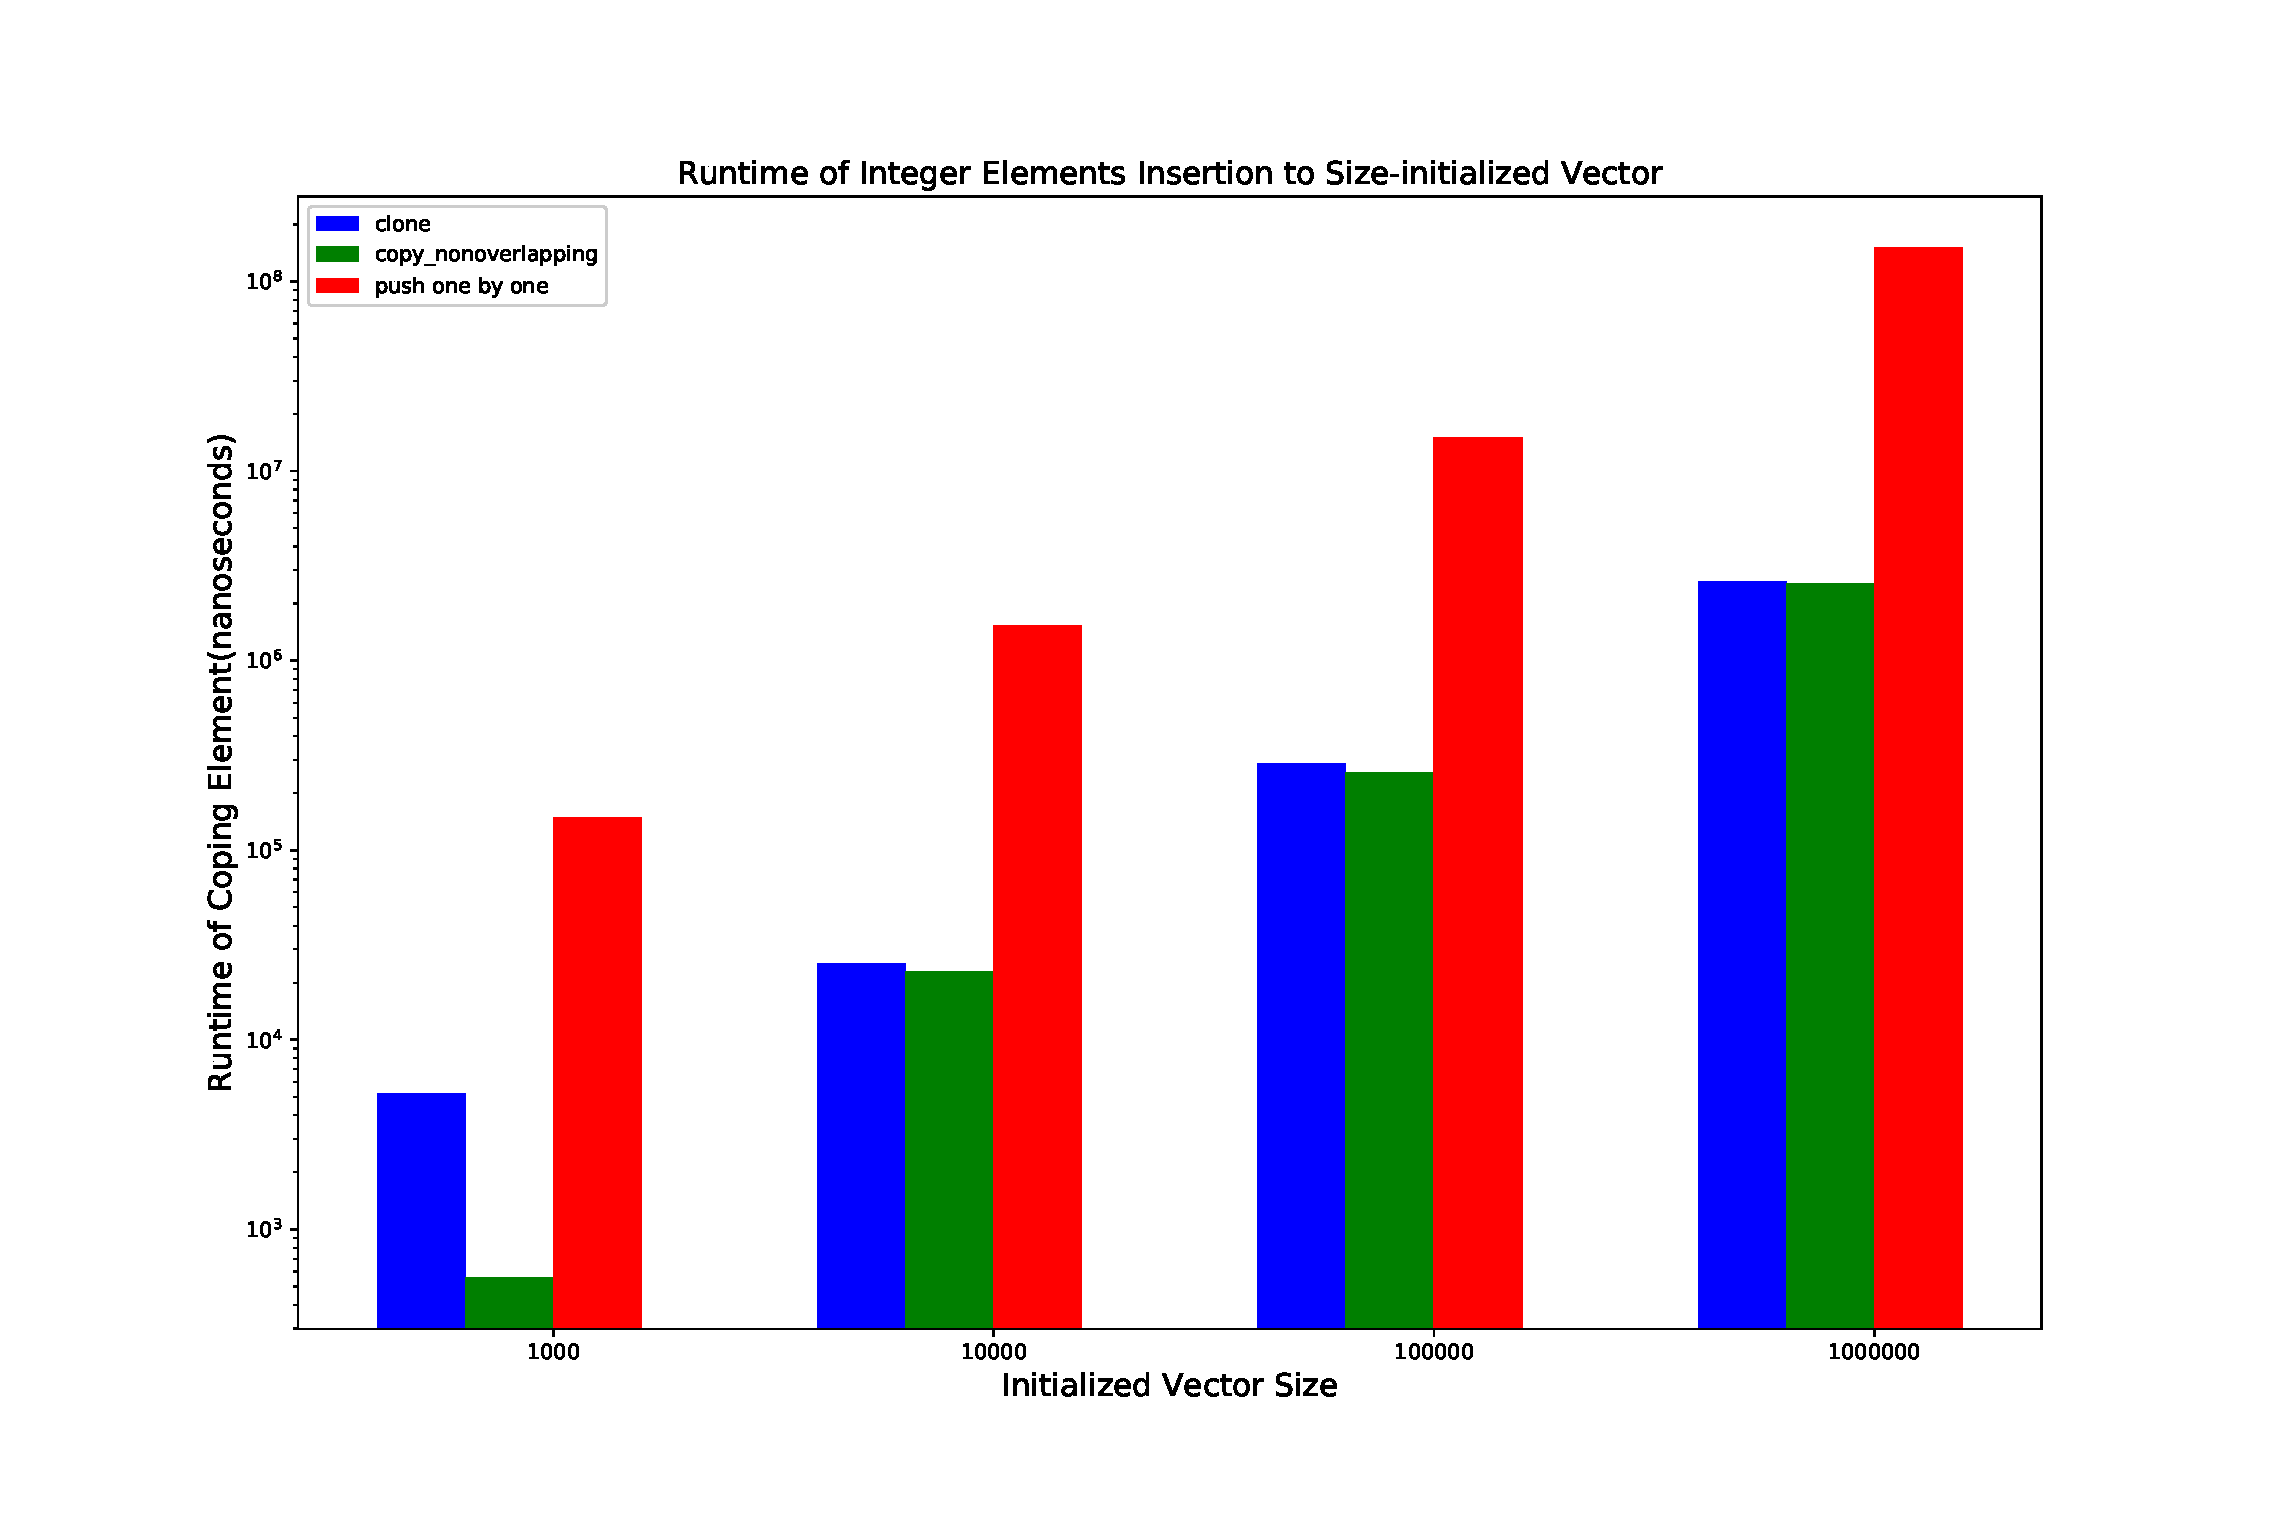
\includegraphics[width=15cm]{rust_various_insertion.eps}
    \caption{Runtime of elements copy from one vector and insertion to the other vector.}
    \label{fig:Sampling}
\end{figure}
\clearpage

\section{Access time to elements in vector}
\label{sec:history}
In this experiment, whether mutability has impacts to operation on the object in terms of runtime performance. 
According to the experiment, there is no difference on accessing to elements of mutable and immutable vector.

\begin{figure}[htb]
    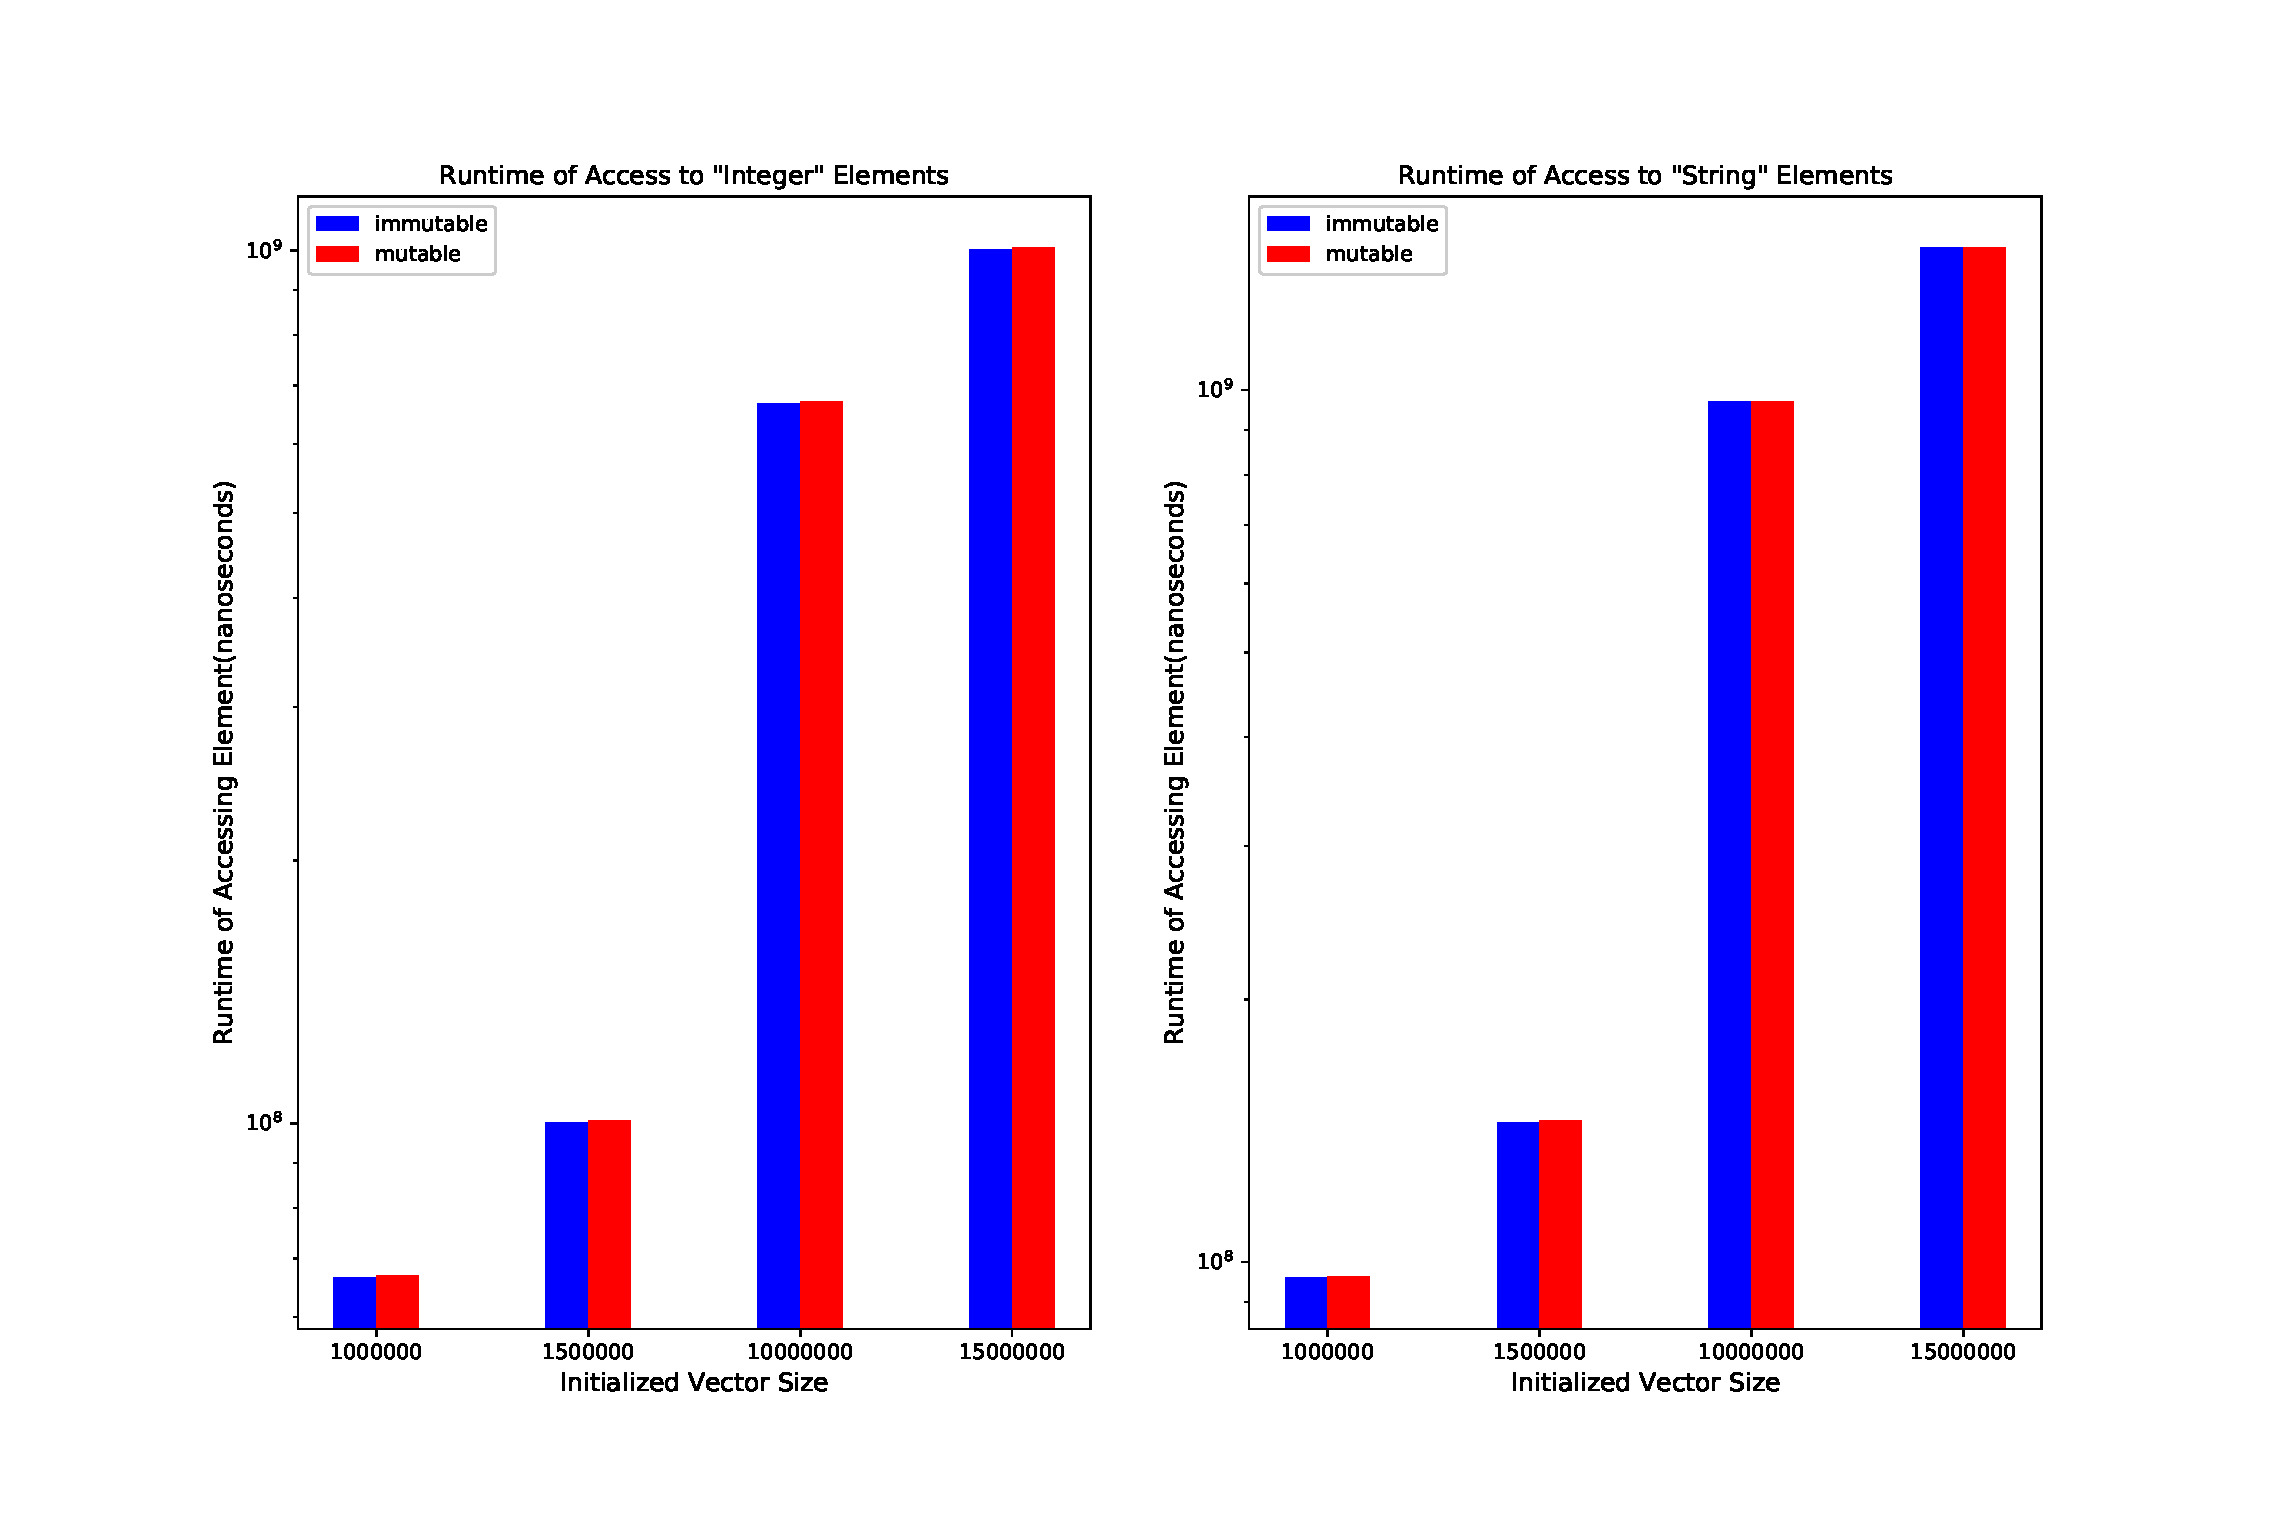
\includegraphics[width=15cm]{rust_various_access.eps}
    \caption{Runtime of elements copy from one vector and insertion to the other vector.}
    \label{fig:Sampling}
\end{figure}



